\hypertarget{funnel-metadynamics-tutorial}{%
\label{funnel-metadynamics-tutorial}}
\hypertarget{Introduction}{%
\subsubsection{Introduction}\label{Introduction}}

Funnel metadynamics (\emph{fun-metaD}) is a molecular dynamics-based method that calculates the absolute binding free energy (ABFE) between a small organic ligand and a protein. It uses the enhanced sampling method metadynamics. To best separate the bound
and unbound phases, as well as increase the rate of convergence of the binding free energy, the exploration of the ligand in 3D space is limited by funnel-shaped
restraints.

\emph{fun-metaD} was originally implemented by Limogelli \emph{et al}~\cite{Limongelli2013}. This tutorial is based on the implementation described by Rhys \emph{et al}~\cite{Evans2020}, and Saleh \emph{et al}~\cite{Saleh2017}. The main difference between the original and later implementations is the functional form of the funnel restraints: the original \emph{fun-metaD} relied on a cone and a cylinder joined to make a funnel using a step function, while the new implementation uses a single
sigmoid function. The Limogelli implementation also requires the protein to be realigned with a reference structure to keep the funnel strictly in place over the binding site, which negatively affects performance. The implementation described here allows the funnel to move with the protein.

A challenge with using \emph{fun-metaD} for ABFE calculations is that it can be difficult to select optimised funnel parameters, and tedious to write multiple input files for PLUMED. To facilitate use of \emph{fun-metaD} by non-experts  BioSimSpace implements automated setup algorithms for selecting funnel parameters, and producing input files. 

By the end of this tutorial, you should understand:
\begin{itemize}
\item The theory that underpins \emph{fun-metaD} calculations.
\item How to set up \emph{fun-metaD} simulations and how to
visualise the funnel restraints.
\item How to analyse the results of a \emph{fun-metaD} simulation.
\end{itemize}

\hypertarget{the-theory}{%
\subsubsection{Theory}\label{the-theory}}

Metadynamics is an enhanced sampling method that biases a simulation
along a chosen set of reaction coordinates, or as MetaD practitioners
call them, collective variables (CVs). This bias is deposited at defined
time intervals and takes the shape of a Gaussian potential.
Investigation of drug binding should involve at least one CV, the distance
from the drug molecule to the protein, where the distance between them
can be biased, causing the drug to unbind. However, that single distance
is degenerate, meaning many different configurations of the drug in 3D
space will not be described by that single distance. It also involves
the exploration of a very large volume, hindering convergence.

\emph{Fun-metaD} gets around both of these problems, restricting the
exploration by using funnel-shaped restraints. The restraints are defined with a 2D coordinates system based on the  two CVs - `projection' and `extent'. The first CV measures the distance along the axis-vector defined by the coordinates of the points $P_{0}$ and $P_{X}$ in the laboratory frame. The second CV measures the distance along a second axis-vector orthogonal to the first axis-vector. See Figure \ref{fig:funnel}. 

\begin{figure}[htp]
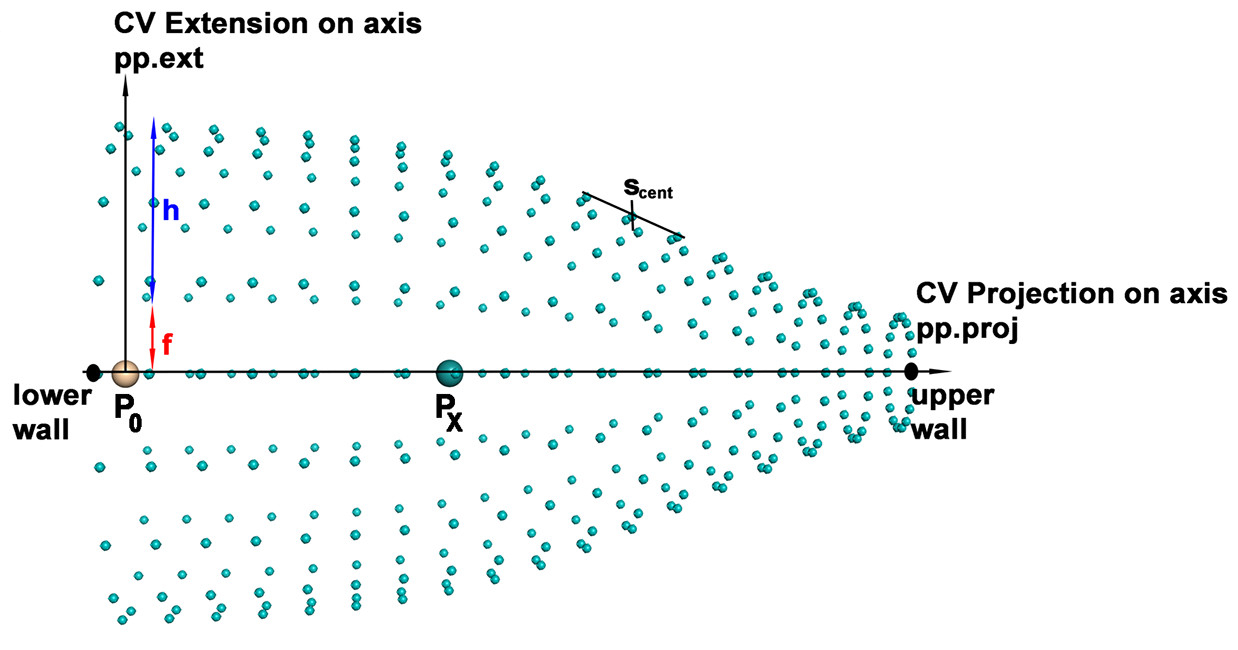
\includegraphics[width=\linewidth]{LIVECOMS/02_funnel_metad/funmetadfig1.jpeg}
\caption{Visualisation of the funnel restraints defined using the CV projection axis and the CV extent axis.}
\label{fig:funnel}
\end{figure}

The funnel parameters $h$ and $f$ controls the maximal and minimal width of the funnel along the extent axis respectively. The smoothness of the transition between maximal and minimal widths along the projection axis is controlled by the parameters $b$ and $x$ that together control the location and steepness of the inflection point located at $S_{cent}$ in fig \ref{fig:funnel}.  All together these parameters define the radius $S$ of the funnel at a given distance $i$ along the projection axis.  

\begin{equation}
S(i) = h\left(\frac{1}{1+b^{b(i-x)}}\right) + f,
\end{equation}

Clearly, there is still some degeneracy in the CVs - the plane
perpendicular to the projection axis is a one-dimensional representation of a two-dimensional space. However, this is a good compromise between having sufficient accuracy for describing the binding of a ligand and the tolerable simulation slowdown of using only two CVs.

In order to have a good separation between the bound and unbound phases for the ABFE estimations, the funnel needs to point \emph{out}, with the narrow end in the solvent,
and away from any protein residues. The BSS automated funnel assignment code does this generally well. Typically the vectors picked for defining the $P_{0}$ and $P_{1}$ points offer an unobstructed exit path for the ligand. It is nonetheless still a good idea to visually check the proposed funnel, especially for new protein systems. This can be done through use of the funnel visualisation functionality within BSS (see below).

The size of the funnel radius has to be determined on a case-by-case basis. The metadynamics code tracks the exploration of the center of mass of the ligand, so the volume that the small molecule will explore is much larger than implied by the visualization of the funnel. There is usually only one binding site and the funnel should enclose only it, excluding other protein features, by setting a small value of $h$. This helps accelerate convergence by preventing the ligand from exploring irrelevant regions in the free energy surface (FES). 

\hypertarget{setupfunmetad}{%
\subsubsection{Setting up funnel metadynamics simulations}\label{setupfunmetad}}

The first tutorial notebook \href{https://github.com/OpenBioSim/biosimspace_tutorials/blob/main/02_funnel_metad/01_bss-fun-metad-setup.ipynb}{01-bss-fun-metad-setup} shows how to set up a BioSimSpace system, parameterizing the protein and the ligand, as well as defining the simulation box, adding water and ions. A funnel is then defined and visualized using NGLview. Finally, directories for the \emph{fun-metaD} simulation are setup and a short 10 ps simulation is run for illustrative purposes.


\begin{figure}[htp]
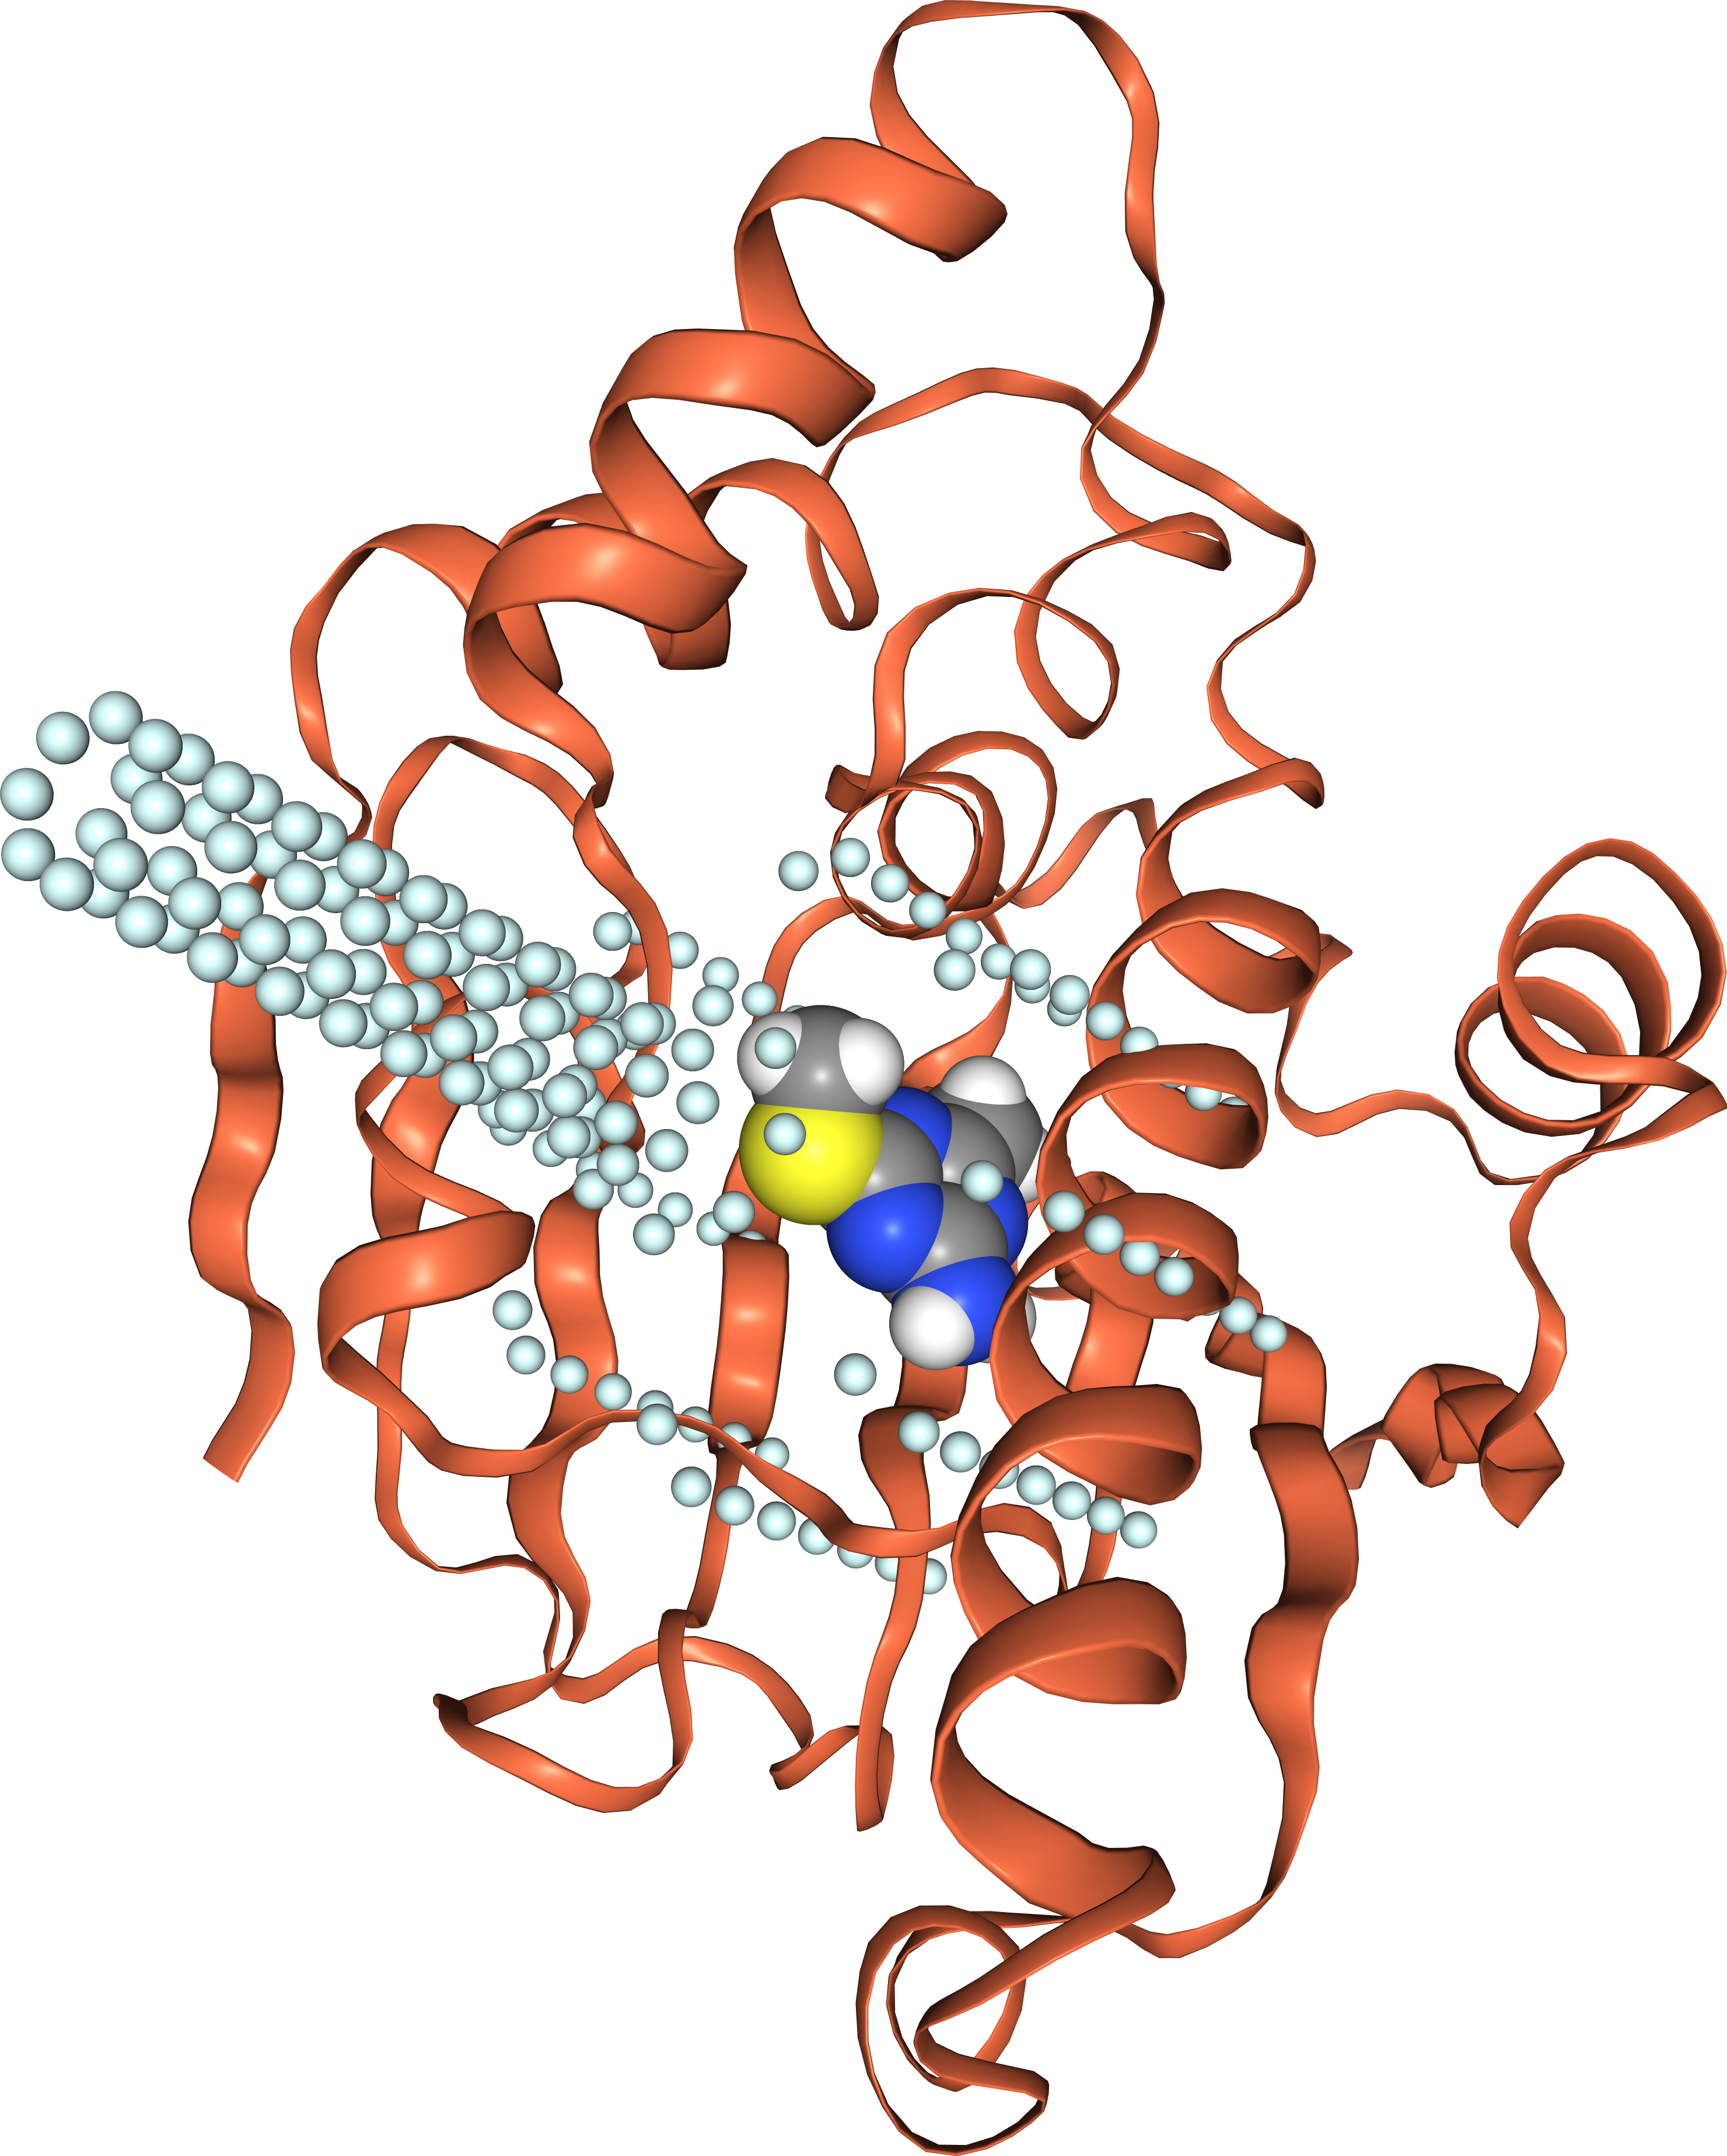
\includegraphics[width=\linewidth]{LIVECOMS/02_funnel_metad/funmetad-hsp90.png}
\caption{Visualisation of funnel restraints autogenerated by BioSimSpace for a HSP90 protein-ligand system.}
\label{fig:fun-hsp90}
\end{figure}

The notebook uses as example a fully solvated HSP90 protein-ligand system originally setup from PDBID:2WI2. 
Figure \ref{fig:fun-hsp90} depicts a rendered funnel overlayed on the HSP90 protein-ligand system in the Jupyter Notebook. The funnel vector is clearly pointing out into the solvent, with no protein residues blocking the way. The default radius is sufficient to encompass the binding site, excluding the rest of the protein.


To obtain converged free energies we recommend simulations of the order of 500 - 2000 ns sampling time. This is best done out of a notebook. For convenience we also \href{https://github.com/OpenBioSim/biosimspace_tutorials/tree/main/02_funnel_metad/example_nodes}{provide with this tutorial} as companion resource an LSF submission script that re-implements the notebook functionality in a set of BioSimSpace nodes.  

\hypertarget{analysis}{%
\subsubsection{Analysing funnel metadynamics simulations}\label{analysis}}

The second notebook of this tutorial  \href{https://github.com/OpenBioSim/biosimspace_tutorials/blob/main/02_funnel_metad/02_bss-fun-metad-analysis.ipynb}{02-bss-fun-metad-analysis} describes how to analyze a funnel metadynamics simulation. The precision of the ABFE estimate derived from a funnel metadynamics run is linked to the convergence of the free energy profile along the collective variables that define the funnel. The notebook uses provided sample trajectories to show how the range of CV values sampled during a trajectory and two-dimensional free energy surfaces can be plotted with the help of \href{https://biosimspace.openbiosim.org/api/index_Notebook.html}{BSS.Notebook}. The notebook also shows how to compute funnel correction terms using BSS, and how to perform convergence analysis of the absolute binding free energies for different trajectories. Selected visualizations generated by the notebook are depicted in Figure~\ref{fig:fun-hsp90-analyses}. 

\begin{figure}[htp]
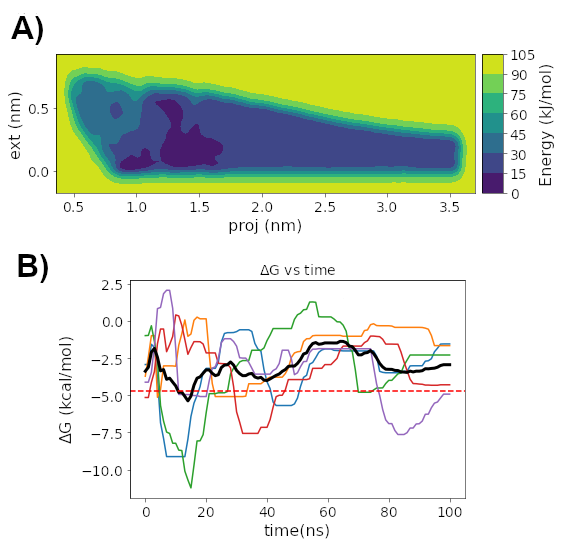
\includegraphics[width=\linewidth]{LIVECOMS/02_funnel_metad/fun-hsp90-analyses.png}
\caption{Selected analyses of funnel metadynamics simulations of the HSP90 protein-ligand system. A) Reconstructed two-dimensional free energy profile from a sample 100 ns trajectory. B) Convergence plots for five replicates of a 100-ns trajectory. The bold black line denotes the mean of the replicates, and the dashed red line the experimental estimate of the absolute binding free energy of the ligand.}
\label{fig:fun-hsp90-analyses}
\end{figure}

